% Options for packages loaded elsewhere
\PassOptionsToPackage{unicode}{hyperref}
\PassOptionsToPackage{hyphens}{url}
\PassOptionsToPackage{dvipsnames,svgnames,x11names}{xcolor}
%
\documentclass[
  letterpaper,
  DIV=11,
  numbers=noendperiod]{scrartcl}

\usepackage{amsmath,amssymb}
\usepackage{iftex}
\ifPDFTeX
  \usepackage[T1]{fontenc}
  \usepackage[utf8]{inputenc}
  \usepackage{textcomp} % provide euro and other symbols
\else % if luatex or xetex
  \usepackage{unicode-math}
  \defaultfontfeatures{Scale=MatchLowercase}
  \defaultfontfeatures[\rmfamily]{Ligatures=TeX,Scale=1}
\fi
\usepackage{lmodern}
\ifPDFTeX\else  
    % xetex/luatex font selection
\fi
% Use upquote if available, for straight quotes in verbatim environments
\IfFileExists{upquote.sty}{\usepackage{upquote}}{}
\IfFileExists{microtype.sty}{% use microtype if available
  \usepackage[]{microtype}
  \UseMicrotypeSet[protrusion]{basicmath} % disable protrusion for tt fonts
}{}
\makeatletter
\@ifundefined{KOMAClassName}{% if non-KOMA class
  \IfFileExists{parskip.sty}{%
    \usepackage{parskip}
  }{% else
    \setlength{\parindent}{0pt}
    \setlength{\parskip}{6pt plus 2pt minus 1pt}}
}{% if KOMA class
  \KOMAoptions{parskip=half}}
\makeatother
\usepackage{xcolor}
\setlength{\emergencystretch}{3em} % prevent overfull lines
\setcounter{secnumdepth}{5}
% Make \paragraph and \subparagraph free-standing
\makeatletter
\ifx\paragraph\undefined\else
  \let\oldparagraph\paragraph
  \renewcommand{\paragraph}{
    \@ifstar
      \xxxParagraphStar
      \xxxParagraphNoStar
  }
  \newcommand{\xxxParagraphStar}[1]{\oldparagraph*{#1}\mbox{}}
  \newcommand{\xxxParagraphNoStar}[1]{\oldparagraph{#1}\mbox{}}
\fi
\ifx\subparagraph\undefined\else
  \let\oldsubparagraph\subparagraph
  \renewcommand{\subparagraph}{
    \@ifstar
      \xxxSubParagraphStar
      \xxxSubParagraphNoStar
  }
  \newcommand{\xxxSubParagraphStar}[1]{\oldsubparagraph*{#1}\mbox{}}
  \newcommand{\xxxSubParagraphNoStar}[1]{\oldsubparagraph{#1}\mbox{}}
\fi
\makeatother


\providecommand{\tightlist}{%
  \setlength{\itemsep}{0pt}\setlength{\parskip}{0pt}}\usepackage{longtable,booktabs,array}
\usepackage{calc} % for calculating minipage widths
% Correct order of tables after \paragraph or \subparagraph
\usepackage{etoolbox}
\makeatletter
\patchcmd\longtable{\par}{\if@noskipsec\mbox{}\fi\par}{}{}
\makeatother
% Allow footnotes in longtable head/foot
\IfFileExists{footnotehyper.sty}{\usepackage{footnotehyper}}{\usepackage{footnote}}
\makesavenoteenv{longtable}
\usepackage{graphicx}
\makeatletter
\def\maxwidth{\ifdim\Gin@nat@width>\linewidth\linewidth\else\Gin@nat@width\fi}
\def\maxheight{\ifdim\Gin@nat@height>\textheight\textheight\else\Gin@nat@height\fi}
\makeatother
% Scale images if necessary, so that they will not overflow the page
% margins by default, and it is still possible to overwrite the defaults
% using explicit options in \includegraphics[width, height, ...]{}
\setkeys{Gin}{width=\maxwidth,height=\maxheight,keepaspectratio}
% Set default figure placement to htbp
\makeatletter
\def\fps@figure{htbp}
\makeatother
% definitions for citeproc citations
\NewDocumentCommand\citeproctext{}{}
\NewDocumentCommand\citeproc{mm}{%
  \begingroup\def\citeproctext{#2}\cite{#1}\endgroup}
\makeatletter
 % allow citations to break across lines
 \let\@cite@ofmt\@firstofone
 % avoid brackets around text for \cite:
 \def\@biblabel#1{}
 \def\@cite#1#2{{#1\if@tempswa , #2\fi}}
\makeatother
\newlength{\cslhangindent}
\setlength{\cslhangindent}{1.5em}
\newlength{\csllabelwidth}
\setlength{\csllabelwidth}{3em}
\newenvironment{CSLReferences}[2] % #1 hanging-indent, #2 entry-spacing
 {\begin{list}{}{%
  \setlength{\itemindent}{0pt}
  \setlength{\leftmargin}{0pt}
  \setlength{\parsep}{0pt}
  % turn on hanging indent if param 1 is 1
  \ifodd #1
   \setlength{\leftmargin}{\cslhangindent}
   \setlength{\itemindent}{-1\cslhangindent}
  \fi
  % set entry spacing
  \setlength{\itemsep}{#2\baselineskip}}}
 {\end{list}}
\usepackage{calc}
\newcommand{\CSLBlock}[1]{\hfill\break\parbox[t]{\linewidth}{\strut\ignorespaces#1\strut}}
\newcommand{\CSLLeftMargin}[1]{\parbox[t]{\csllabelwidth}{\strut#1\strut}}
\newcommand{\CSLRightInline}[1]{\parbox[t]{\linewidth - \csllabelwidth}{\strut#1\strut}}
\newcommand{\CSLIndent}[1]{\hspace{\cslhangindent}#1}

\usepackage{float}
\usepackage{tabularray}
\usepackage[normalem]{ulem}
\usepackage{graphicx}
\UseTblrLibrary{booktabs}
\UseTblrLibrary{rotating}
\UseTblrLibrary{siunitx}
\NewTableCommand{\tinytableDefineColor}[3]{\definecolor{#1}{#2}{#3}}
\newcommand{\tinytableTabularrayUnderline}[1]{\underline{#1}}
\newcommand{\tinytableTabularrayStrikeout}[1]{\sout{#1}}
\KOMAoption{captions}{tableheading}
\makeatletter
\@ifpackageloaded{caption}{}{\usepackage{caption}}
\AtBeginDocument{%
\ifdefined\contentsname
  \renewcommand*\contentsname{Table of contents}
\else
  \newcommand\contentsname{Table of contents}
\fi
\ifdefined\listfigurename
  \renewcommand*\listfigurename{List of Figures}
\else
  \newcommand\listfigurename{List of Figures}
\fi
\ifdefined\listtablename
  \renewcommand*\listtablename{List of Tables}
\else
  \newcommand\listtablename{List of Tables}
\fi
\ifdefined\figurename
  \renewcommand*\figurename{Figure}
\else
  \newcommand\figurename{Figure}
\fi
\ifdefined\tablename
  \renewcommand*\tablename{Table}
\else
  \newcommand\tablename{Table}
\fi
}
\@ifpackageloaded{float}{}{\usepackage{float}}
\floatstyle{ruled}
\@ifundefined{c@chapter}{\newfloat{codelisting}{h}{lop}}{\newfloat{codelisting}{h}{lop}[chapter]}
\floatname{codelisting}{Listing}
\newcommand*\listoflistings{\listof{codelisting}{List of Listings}}
\makeatother
\makeatletter
\makeatother
\makeatletter
\@ifpackageloaded{caption}{}{\usepackage{caption}}
\@ifpackageloaded{subcaption}{}{\usepackage{subcaption}}
\makeatother

\ifLuaTeX
  \usepackage{selnolig}  % disable illegal ligatures
\fi
\usepackage{bookmark}

\IfFileExists{xurl.sty}{\usepackage{xurl}}{} % add URL line breaks if available
\urlstyle{same} % disable monospaced font for URLs
\hypersetup{
  pdftitle={Analyzing Strawberry Pricing Strategies Across Canadian Vendors},
  pdfauthor={Tianning He},
  colorlinks=true,
  linkcolor={blue},
  filecolor={Maroon},
  citecolor={Blue},
  urlcolor={Blue},
  pdfcreator={LaTeX via pandoc}}


\title{Analyzing Strawberry Pricing Strategies Across Canadian
Vendors\thanks{Code and data are available at:
https://github.com/HeTianning/The-price-of-strawberries}}
\usepackage{etoolbox}
\makeatletter
\providecommand{\subtitle}[1]{% add subtitle to \maketitle
  \apptocmd{\@title}{\par {\large #1 \par}}{}{}
}
\makeatother
\subtitle{Price Variations Driven by Supplier Strategies and Seasonal
Demand in Canadian Grocery Markets}
\author{Tianning He}
\date{November 25, 2024}

\begin{document}
\maketitle
\begin{abstract}
This study investigates the pricing of strawberries across eight major
suppliers in Canada: Voila, T\&T, Loblaws, No Frills, Metro, Galleria,
Walmart, and Save-On-Foods. Using a dataset containing variables such as
current price, old price, and month, a Bayesian regression model was
applied to analyze the relationships between pricing strategies,
seasonal trends, and vendor-specific practices. Results reveal
significant price variation among suppliers, with old price showing a
strong positive correlation with current price, reflecting the impact of
prior pricing strategies on current prices. Seasonal trends captured by
the month variable indicate subtle but consistent fluctuations in
pricing, highlighting the influence of supply and demand dynamics. These
findings provide actionable insights into supplier-specific pricing
strategies and market behavior, offering valuable guidance to consumers
and stakeholders in the Canadian strawberry market.
\end{abstract}


\section{Introduction}\label{introduction}

Strawberries are one of the most important small berries in Canada and
the United States(Macoun and McCubbin (1919)), and pricing of
strawberries in the Canadian retail market varies widely due to factors
such as supplier strategies, promotional practices, and temporal trends.
This investigation examines the determinants of strawberry prices,
focusing on differences between different suppliers, the role of
discounts, and seasonal effects. By utilizing a Bayesian linear
regression model, the study examines the relationship between key
predictors (supplier, original price, promotion, and time) and the
current price of strawberries. The Bayesian approach not only provides
parameter estimates but also quantifies uncertainty, thus providing a
nuanced understanding of price dynamics in competitive and seasonal
markets.

The main objective of this analysis is to estimate and explain the
factors that influence retail strawberry prices in Canada. The dependent
variable current price reflects the Canadian dollar price per pound of
strawberries. The key predictors include supplier identity
(categorical), which captures supplier-specific pricing strategies; old
price (continuous), which represents the original price before
promotion, and month (continuous), which captures temporal or seasonal
trends(Hodgdon et al. (2024)). By modeling these relationships, the
study aims to quantify how these variables affect pricing and explore
their combined impact on strawberry price changes.

The results show significant differences in supplier-specific pricing
strategies, with Metro offering higher prices than other suppliers,
consistent with its premium market positioning. Time trends indicate a
gradual but consistent increase in strawberry prices over time, possibly
reflecting seasonal demand or inflationary pressures. Furthermore, the
analysis shows a strong relationship between original and discounted
prices, suggesting that promotional pricing generally preserves relative
price hierarchies among suppliers. Bayesian models confirm strong
convergence and robust posterior estimates, ensuring the reliability of
these findings.

Understanding the factors driving strawberry prices is critical for both
consumers and retailers. For suppliers, insights into pricing dynamics
can inform strategies to optimize revenue while remaining competitive.
For consumers, this analysis provides valuable information to navigate
the market, highlighting opportunities to save costs by selecting
suppliers or purchasing during promotions. More broadly, these findings
contribute to the study of the fresh produce market, where pricing is
influenced by a complex interaction between supplier strategies,
seasonal supply, and consumer behavior. This study lays the foundation
for future research that could incorporate additional factors, such as
geographic differences or organic certification, to further enrich our
understanding of pricing dynamics in Canadian retail.

The rest of the paper is structured as follows. Section~\ref{sec-data}
describes the data collection process, including data sources, sampling
strategy, and preprocessing steps taken to ensure data quality.
Section~\ref{sec-model} outlines the methodological framework, focusing
on the Bayesian linear regression model, its formulation, and diagnostic
checks. Section~\ref{sec-result} presents the main findings of the
analysis, focusing on specific supplier pricing strategies, seasonal
trends, and the impact of sales and promotions on strawberry prices.
Section~\ref{sec-discussion} discusses the implications of these
findings, placing them in the broader context of consumer behavior and
supplier strategies in the fresh produce market.

\section{Data}\label{sec-data}

To conduct the analysis, \texttt{R}, a versatile statistical programming
language, was utilized for simulating, testing, downloading, cleaning,
and modeling data (R Core Team 2023). Several powerful libraries
supported various stages of the analysis. The \texttt{tidyverse} package
suite (Wickham et al. 2019), which includes \texttt{dplyr} for data
manipulation and \texttt{ggplot2} for visualization, was central to
handling and exploring the dataset. Data cleaning and structuring were
enhanced using \texttt{janitor}, while \texttt{arrow} facilitated
efficient handling of large datasets by enabling seamless reading and
writing of data (Apache Arrow 2021). The \texttt{here} package
streamlined file management, ensuring robust and reproducible workflows
(Müller 2020).

Visualization and reporting were further supported by \texttt{knitr}
(Xie 2021), which enabled dynamic report generation, and
\texttt{modelsummary} (Arel-Bundock 2022), which provided
professional-quality summaries for statistical models. Bayesian modeling
and advanced statistical analysis were conducted using \texttt{rstanarm}
(Goodrich et al. 2022), while posterior diagnostics and visualizations
were enhanced with \texttt{bayesplot} (Gelman, Gabry, et al. 2021).
Testing and quality assurance of code were carried out with
\texttt{testthat} (Wickham 2011), ensuring the reliability and
reproducibility of results.

By integrating these libraries the analysis leveraged a comprehensive
ecosystem of tools, demonstrating the strength and flexibility of R in
handling complex data-driven research workflows.

\subsection{Overview}\label{overview}

The data for this analysis was provided by Project Hammer (Filipp 2024),
which was collected through a process of scraping website UI screens
from vendors within the Toronto community. It contains data on product
details (e.g., product name, brand, current and old price, and unit of
product) for 8 different grocery stores (Voila, T\&T, Loblaws, No
Frills, Metro, Galleria, Walmart Canada, and Save-On-Foods). Project
Hammer's data is available from February 28, 2024, and since the data is
collected by extracting information from grocery store websites, there
may be missing data, as discussed in appendix. Through the method of
screen scraping, the raw data is intended to measure and reflect grocery
store vendor decisions and product pricing trends.

For this analysis, the eight vendors - Voila, T\&T, Loblaws, No Frills,
Metro, Galleria, Walmart Canada, and Save-On-Foods - and their pricing
for strawberries were considered. The variable ``price'' for each
supplier in this analysis reflects the current price of their product at
the time the data was downloaded.

\subsection{Measurement}\label{measurement}

The dataset provides a detailed and structured framework for analyzing
strawberry pricing dynamics in the Canadian market, offering critical
insights into supplier-specific pricing strategies and seasonal trends.
The central variable of interest is the current price, a continuous
measure representing the price of strawberries in Canadian dollars at
the time of observation. This variable acts as the dependent variable in
the analysis and reflects real-time vendor pricing decisions, including
adjustments for promotions, sales, or other market-driven factors. The
current price is essential for understanding how vendors position their
products in response to competition and consumer demand.

Complementing this, the dataset includes the old price, another
continuous variable that captures the price of strawberries before any
discounts or promotional offers. The old price serves as a benchmark for
evaluating vendor markdowns, sales strategies, and pricing flexibility.
By calculating the difference between the old price and the current
price, the analysis can quantify the extent and frequency of price
reductions, revealing patterns in promotional behavior. For instance,
larger discounts may indicate aggressive marketing tactics during
periods of high supply or low demand. Together, current and old prices
allow for a nuanced exploration of how pricing evolves over time and in
response to market conditions.

The dataset also incorporates vendor as a categorical variable,
identifying one of eight major suppliers: Voila, T\&T, Loblaws, No
Frills, Metro, Galleria, Walmart, and Save-On-Foods. This variable is
pivotal for inter-vendor comparisons, enabling the analysis to uncover
unique pricing strategies, competitive behaviors, and market
segmentation. By examining differences in pricing across these
suppliers, the analysis can identify which vendors consistently offer
lower prices, adopt aggressive discounting practices, or align their
pricing with premium branding.

Another critical variable is month, recorded as a numeric measure that
captures the time of observation on a monthly scale. This variable
facilitates the investigation of seasonal trends, allowing for the
analysis of how strawberry prices fluctuate throughout the year.
Seasonal dynamics may reflect changes in supply (e.g., peak harvest
periods), demand (e.g., holidays or special occasions), and
vendor-specific pricing adjustments. By integrating month with pricing
data, the analysis can identify whether prices tend to peak or dip
during specific times of the year and how these patterns vary among
vendors.

These variables collectively provide a rich dataset for conducting both
granular and aggregate analyses of strawberry pricing. The inclusion of
current and old prices enables an in-depth exploration of
vendor-specific pricing adjustments, while the categorical vendor
variable allows for competitive benchmarking across suppliers. The month
variable introduces a temporal dimension, facilitating the study of
seasonal effects on pricing. Together, this dataset offers a
comprehensive foundation for understanding the complex interplay between
market forces, supplier behavior, and seasonal trends, yielding
actionable insights for consumers seeking the best value and suppliers
aiming to optimize their pricing strategies.

\subsection{Outcome variable}\label{outcome-variable}

The primary outcome variable in this study is current price, which
represents the current price of strawberries in Canadian dollars. This
continuous variable serves as the dependent variable and captures the
prices consumers pay at the point of purchase, reflecting
vendor-specific pricing strategies and promotional adjustments.
Additionally, old price is included as a secondary outcome variable,
representing the original price before any discounts. The relationship
between these two variables highlights the frequency and magnitude of
price reductions, offering insights into vendor markdown strategies.

The analysis focuses on understanding how current price varies with
factors such as vendor and month. The categorical variable vendor
identifies the supplier and captures differences in pricing strategies
across eight vendors, ranging from premium to budget-focused retailers.
These variations help reveal how suppliers target different market
segments through pricing. The numeric variable month enables the
exploration of seasonal trends and temporal fluctuations, reflecting how
supply and demand dynamics influence pricing throughout the year.

By examining both current price and old price, the study provides a
detailed view of promotional activity and vendor behavior. A significant
gap between the two prices indicates aggressive promotional strategies,
while minimal differences suggest stable pricing policies. Additionally,
incorporating the month variable allows for insights into seasonal peaks
or dips in strawberry prices, such as higher prices during off-seasons
or lower prices during harvest months. Together, these variables offer a
comprehensive understanding of strawberry pricing dynamics in Canada's
retail market, helping inform consumer choices and vendor pricing
strategies.

\begin{figure}

\centering{

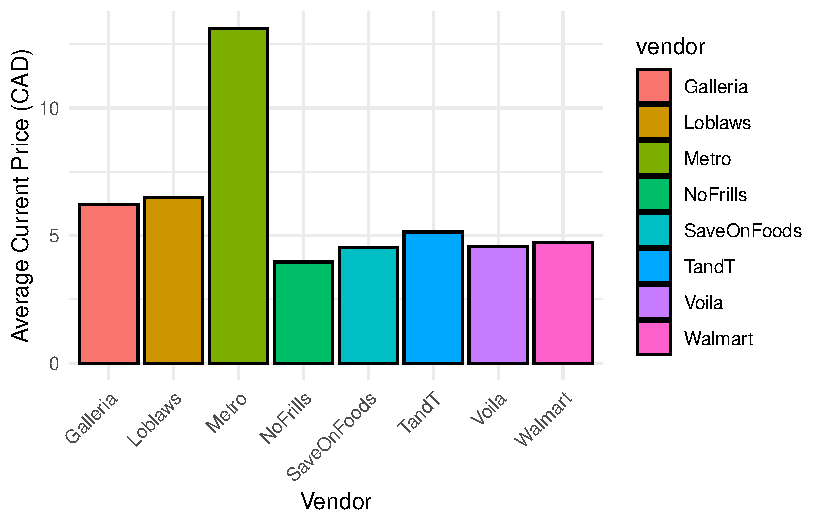
\includegraphics{paper_files/figure-pdf/fig-currentpricebyvendor-1.pdf}

}

\caption{\label{fig-currentpricebyvendor}Average Current Price by
Vendor}

\end{figure}%

The graph(Figure~\ref{fig-currentpricebyvendor}) illustrates the average
current price of strawberries across various vendors, highlighting
significant price variations. \texttt{Metro} stands out with the highest
average price, indicating a focus on premium offerings or higher-quality
products, while \texttt{No\ Frills} and \texttt{Save-On-Foods} have the
lowest prices, appealing to cost-conscious shoppers. Vendors like
\texttt{Loblaws}, \texttt{T\&T}, and \texttt{Voila} fall into the
mid-range pricing category, suggesting a balance between affordability
and quality. These differences reflect distinct market strategies, with
premium vendors targeting quality-focused consumers and budget-friendly
vendors catering to price-sensitive customers. The data provides
valuable insights for consumers to make informed purchasing decisions
and for vendors to refine their pricing strategies to better compete in
their respective market segments.

\begin{figure}

\centering{

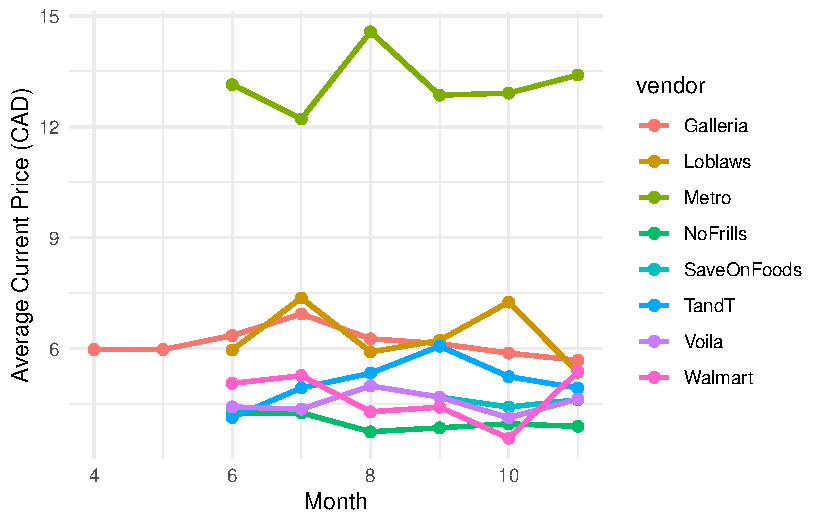
\includegraphics{paper_files/figure-pdf/fig-monthlytrend-1.pdf}

}

\caption{\label{fig-monthlytrend}Monthly Trend of Current Prices by
Vendor}

\end{figure}%

This graph(Figure~\ref{fig-monthlytrend}) shows the monthly trend of
average current strawberry prices across different vendors over several
months. \texttt{Metro} consistently exhibits the highest prices, with
noticeable fluctuations, peaking in mid-year, indicating potential
seasonal effects or changes in supply and demand. In contrast,
budget-friendly vendors like \texttt{No\ Frills} and
\texttt{Save-On-Foods} maintain the lowest prices, demonstrating pricing
stability aimed at cost-conscious consumers. Mid-range vendors such as
\texttt{Loblaws}, \texttt{T\&T}, and \texttt{Voila} show relatively
stable but slightly variable trends, with occasional peaks suggesting
targeted pricing adjustments. Overall, the graph highlights clear
segmentation among vendors, with premium vendors like \texttt{Metro}
adapting dynamically to market conditions, while budget vendors maintain
consistent affordability. This trend could reflect differing business
strategies to cater to diverse consumer preferences.

\subsection{Predictor variables}\label{predictor-variables}

Predictor Variables: Exploring Factors Influencing Strawberry Prices

\begin{enumerate}
\def\labelenumi{\arabic{enumi}.}
\tightlist
\item
  Vendor
\end{enumerate}

The vendor variable is categorical, identifying the supplier of
strawberries. Each vendor employs unique pricing strategies, leading to
significant variability in pricing across the eight vendors (Voila,
T\&T, Loblaws, No Frills, Metro, Galleria, Walmart, and Save-On-Foods).
Premium vendors like Metro and Galleria tend to target quality-conscious
consumers, reflected in their higher average prices. In contrast,
budget-oriented vendors like No Frills and Save-On-Foods maintain lower
prices to attract cost-sensitive shoppers. The variability in pricing,
shown through boxplots, highlights how vendor identity influences price
distributions and captures the strategic segmentation of the Canadian
strawberry market.

\begin{enumerate}
\def\labelenumi{\arabic{enumi}.}
\setcounter{enumi}{1}
\tightlist
\item
  Old and Current Prices
\end{enumerate}

The dataset includes two continuous price variables: old price (original
price) and current price (price after any promotions or discounts). The
difference between these two variables provides insights into
promotional behavior and markdown strategies. Vendors like No Frills and
Save-On-Foods typically show small gaps between old price and current
price, suggesting limited use of deep discounts, whereas Metro and
Walmart exhibit larger gaps, reflecting more aggressive promotional
activity. Boxplots comparing old price and current price by vendor
demonstrate how discounts influence consumer pricing perceptions and
vendor competition.

\begin{enumerate}
\def\labelenumi{\arabic{enumi}.}
\setcounter{enumi}{2}
\tightlist
\item
  Month (month)
\end{enumerate}

The month variable is numeric, capturing the month of observation.
Seasonal patterns play a crucial role in strawberry pricing, with supply
and demand fluctuations driving price variability. For instance, prices
may drop during peak harvest months and increase during off-season
periods when strawberries are scarce. Line charts tracking average
monthly prices show clear temporal trends, with peaks and dips aligning
with these seasonal dynamics. By analyzing month in combination with
other predictors, this variable helps uncover how vendors adjust pricing
strategies to reflect seasonal demand and supply conditions.

The interplay of vendor, old price, current price, and month allows for
a more comprehensive analysis of pricing strategies. For example,
vendors like Metro may use larger discounts (old price vs.~current
price) during peak seasons to maintain competitiveness, while budget
vendors like No Frills may maintain consistent pricing throughout the
year. A combined analysis using bar charts and line plots highlights how
vendor strategies vary with time, providing insights into the dynamic
nature of strawberry pricing.

The inclusion of variables like vendor, old price, current price, and
month enriches the analysis by offering multiple perspectives on pricing
strategies. Vendor captures the segmentation of suppliers into premium
and budget categories, reflecting strategic decisions about market
positioning. The dual price variables (old price and current price)
allow for a deeper understanding of promotional activity and highlight
the extent to which vendors rely on discounts to influence consumer
behavior.

The addition of month introduces a temporal dimension, enabling the
analysis of seasonal trends that are common in agricultural markets.
Combining these predictors provides a holistic view of pricing dynamics,
revealing how vendors adapt to seasonal supply fluctuations, consumer
demand, and competitive pressures.

By leveraging these predictor variables, the study offers actionable
insights into how strawberry prices are shaped by market forces, vendor
decisions, and seasonal trends. These findings are crucial for both
consumers seeking to optimize purchases and vendors aiming to refine
their pricing strategies to remain competitive.

\section{Model}\label{sec-model}

\subsection{Purpose of the Model}\label{purpose-of-the-model}

The purpose of this model is to identify and quantify the factors
influencing the current price of strawberries across various vendors in
Canada. The analysis evaluates how key predictors, such as vendor,
original price, month, and their interactions, affect pricing.
Specifically, the model aims to:

\begin{itemize}
\tightlist
\item
  Quantify the impact of each predictor (e.g., vendor, original price,
  and month) on strawberry prices.
\item
  Analyze how the gap between original (\texttt{old\_price}) and
  discounted (\texttt{current\_price}) prices varies across vendors.
\item
  Examine seasonal trends in strawberry prices to identify periods of
  high or low prices.
\item
  Provide actionable insights into vendor pricing strategies and market
  dynamics.
\end{itemize}

\subsection{Model Description}\label{model-description}

The chosen model is a \textbf{Bayesian linear regression model}, which
builds on the simplicity of traditional linear regression while
incorporating the Bayesian framework. This allows for probabilistic
insights and robust uncertainty quantification, making it well-suited
for analyzing the factors driving strawberry prices. Further background
details and diagnostics are included in
Appendix~\ref{sec-model-details}.

\textbf{Predictors in the Model}

\begin{itemize}
\item
  \textbf{Vendor (\texttt{vendor})}: A categorical variable identifying
  the supplier of strawberries. Different vendors adopt distinct pricing
  strategies that influence strawberry prices.
\item
  \textbf{Original Price (\texttt{old\_price})}: A continuous variable
  representing the original price of strawberries before discounts or
  promotions. This variable reflects vendor-specific baseline pricing
  strategies.
\item
  \textbf{Month (\texttt{month})}: A numeric variable capturing the
  observation month, enabling the analysis of seasonal trends and
  time-based fluctuations.
\item
  \textbf{Price Gap (\texttt{old\_price\ -\ current\_price})}: A derived
  variable quantifying the magnitude of discounts or markdowns applied
  by vendors.
\end{itemize}

\textbf{Model set-up}

The Bayesian linear regression model is expressed as:

{[} y\_i = \beta\emph{0 + \beta}\{\text{vendor}{[}i{]}\} +
\beta\emph{\{\text{old\_price}\} \cdot x}\{\text{old\_price}{[}i{]}\} +
\beta\emph{\{\text{month}\} \cdot x}\{\text{month}{[}i{]}\} +
\epsilon\_i {]}

where

\begin{itemize}
\tightlist
\item
  \(y_i\): Current price (\texttt{current\_price}) of strawberries for
  observation \(i\) (dependent variable).\\
\item
  \(\beta_0\): Intercept, representing the baseline price (reference
  vendor, average original price, and earliest month).\\
\item
  \(\beta_{\text{vendor}[i]}\): Vendor-specific effect, capturing how
  each supplier's prices deviate from the baseline vendor.\\
\item
  \(\beta_{\text{old\_price}}\): Effect of the original price,
  representing how the initial pricing influences the current price.\\
\item
  \(\beta_{\text{month}}\): Effect of the observation month, capturing
  seasonal or temporal trends in strawberry pricing.\\
\item
  \(\epsilon_i\): Residual error, accounting for variability not
  explained by the predictors.
\end{itemize}

\textbf{Priors in the Bayesian Framework}

For the coefficients (\(\beta\)):

{[} \beta \sim \text{Normal}(0, 2.5) {]}

For the residual standard deviation (\(\sigma\)):

{[} \sigma \sim \text{Exponential}(1) {]}

The priors in this analysis reflect reasonable assumptions about the
relationships between predictors and strawberry prices. Coefficients
\((\beta)\) are assigned normal priors \((\operatorname{Normal}(0,2.5)\)
) to reflect the expectation that most effects are small and centered
around zero, with moderate variability. For example,
\(\beta_{\text {old_price }}\) is expected to be positive, reflecting
the influence of original prices on current prices, while
\(\beta_{\text {month }}\) accounts for typically small seasonal pricing
effects. The intercept \(\left(\beta_0\right)\) also follows a Normal
\((0,2.5)\), assuming the baseline price is near zero with moderate
deviations. Finally, the residual standard deviation \((\sigma)\) is
given an exponential prior \((\operatorname{Exponential}(1))\) to ensure
positivity and account for variability not captured by the predictors.

We run the model in R (R Core Team 2023) using the \texttt{rstanarm}
package of Goodrich et al. (2022). We use the default priors from
\texttt{rstanarm}.

\subsection{Model justification}\label{model-justification}

A Bayesian linear regression model is a suitable approach for this
analysis because it balances simplicity, interpretability, and
flexibility while quantifying uncertainty in parameter estimates. This
model is particularly effective for exploring the continuous outcome
variable, current\_price, and its relationship with predictors such as
vendor, month, and original price (old price). Unlike traditional linear
regression, which assumes a deterministic relationship between
predictors and the outcome, the Bayesian framework provides posterior
distributions for all parameters, enabling richer and more nuanced
inferences. This approach allows us to incorporate prior knowledge,
account for uncertainty, and provide probabilistic insights into
strawberry pricing.

The Bayesian framework also handles sparse or imbalanced data
effectively by leveraging prior distributions to stabilize parameter
estimates. For example, when certain vendors have fewer observations,
the priors prevent overfitting and provide regularized estimates, making
the model robust to variability in data distribution. This ensures
reliable insights into vendor-specific pricing strategies, seasonal
trends, and the influence of baseline (old price) on observed (current
price) prices.

Benefits of Using Bayesian Regression:

\begin{enumerate}
\def\labelenumi{\arabic{enumi}.}
\item
  \textbf{Uncertainty Quantification}:

  \begin{itemize}
  \tightlist
  \item
    The Bayesian approach provides posterior distributions for each
    parameter, allowing for uncertainty quantification. For example, the
    posterior distribution of \(\beta_{\text{vendor}}\) helps quantify
    the uncertainty around vendor-specific pricing effects.
  \end{itemize}
\item
  \textbf{Incorporating Prior Knowledge}:

  \begin{itemize}
  \tightlist
  \item
    Priors enable the incorporation of domain knowledge into the
    analysis. For instance:

    \begin{itemize}
    \tightlist
    \item
      \(\beta_{\text{vendor}}\): Reflects the expectation that most
      vendor effects are close to zero, with some deviations.
    \item
      \(\beta_{\text{month}}\): Captures small but meaningful seasonal
      effects.
    \item
      \(\beta_{\text{old\_price}}\): Represents the assumption that
      higher original prices lead to higher observed prices.
    \end{itemize}
  \end{itemize}
\item
  \textbf{Handling Sparse Data}:

  \begin{itemize}
  \tightlist
  \item
    Bayesian models stabilize estimates when some categories (e.g.,
    certain vendors) have fewer observations. Priors regularize the
    estimates, reducing the risk of overfitting.
  \end{itemize}
\item
  \textbf{Probabilistic Insights}:

  \begin{itemize}
  \tightlist
  \item
    Posterior distributions provide credible intervals, making it easier
    to interpret parameter estimates. For instance, a 95\% credible
    interval for \(\beta_{\text{old\_price}}\) of \([0.8, 1.2]\) means
    there is a 95\% probability that the original price effect lies
    within this range.
  \end{itemize}
\end{enumerate}

\subsection{Choice of Predictors}\label{choice-of-predictors}

\begin{enumerate}
\def\labelenumi{\arabic{enumi}.}
\tightlist
\item
  Vendor
\end{enumerate}

\begin{itemize}
\item
  \textbf{Role}: The vendor variable is categorical, capturing
  supplier-specific pricing strategies. Each vendor adopts distinct
  pricing approaches based on branding, market positioning, and target
  demographics.
\item
  \textbf{Importance}: By including this variable, the model quantifies
  how much each vendor's prices deviate from the baseline vendor,
  providing insights into vendor-specific strategies and market
  segmentation.
\end{itemize}

\begin{enumerate}
\def\labelenumi{\arabic{enumi}.}
\setcounter{enumi}{1}
\tightlist
\item
  Month
\end{enumerate}

\begin{itemize}
\item
  \textbf{Role}: The numeric \texttt{month} variable captures seasonal
  trends in strawberry pricing. This allows the model to account for
  temporal effects, such as higher prices during off-seasons or lower
  prices during harvest periods.
\item
  \textbf{Importance}: Including \texttt{month} helps the model identify
  recurring seasonal patterns, enabling a better understanding of
  time-based price fluctuations.
\end{itemize}

\begin{enumerate}
\def\labelenumi{\arabic{enumi}.}
\setcounter{enumi}{2}
\tightlist
\item
  Original Price
\end{enumerate}

\begin{itemize}
\item
  \textbf{Role}: The continuous variable \texttt{old\_price} represents
  the baseline price before any discounts or promotions. This predictor
  captures the relationship between promotional activity and observed
  prices.
\item
  \textbf{Importance}: Including this variable enables the model to
  assess how the gap between \texttt{old\_price} and
  \texttt{current\_price} varies across vendors and time, providing
  insights into promotional strategies and pricing adjustments.
\end{itemize}

The Bayesian linear regression model is particularly suited for
analyzing strawberry pricing as it allows for robust, interpretable, and
probabilistic inferences. By including predictors such as vendor, month,
and original price, the model captures vendor-specific pricing
strategies, seasonal trends, and promotional behaviors. The chosen
priors reflect realistic expectations about the predictors' effects,
ensuring the model's estimates are stable and reliable. This approach
provides a comprehensive framework for understanding strawberry pricing
dynamics in the Canadian market.

\section{Results}\label{sec-result}

Our results are summarized in Table~\ref{tbl-modelresults}.

The Bayesian linear regression model provides valuable insights into the
factors affecting strawberry prices (\(\text{current\_price}\)) across
Canadian vendors. The results reveal significant differences in vendor
pricing strategies, seasonal trends, and the relationship between
original and current prices. The intercept (\(\beta_0 = 1.52\), SE =
0.66) represents the baseline price for the reference vendor when all
predictors are at their baseline levels. This suggests that the
reference vendor's average price is modest compared to others.

Vendor coefficients highlight pricing diversity, with \textbf{Metro}
charging significantly higher prices (\(\beta_{\text{Metro}} = 7.50\),
SE = 0.59) compared to the reference vendor, consistent with its premium
market positioning. In contrast, budget-friendly vendors such as
\textbf{No Frills} (\(\beta = -0.81\), SE = 0.62) and
\textbf{Save-On-Foods} (\(\beta = -1.00\), SE = 0.63) exhibit lower
prices, catering to cost-conscious consumers. Mid-tier vendors,
including \textbf{Voila}, \textbf{T\&T}, and \textbf{Walmart}, show
smaller negative effects, reflecting competitive but accessible pricing
strategies.

The model also uncovers seasonal trends, with a small but positive
effect of \(\text{month}\) (\(\beta_{\text{month}} = 0.05\), SE = 0.04).
Prices appear to gradually increase over time, likely due to seasonal
supply and demand fluctuations or inflation. This aligns with the
seasonal nature of fresh produce, where prices typically rise during
off-seasons when supply is limited. Additionally, the strong
relationship between \(\text{old\_price}\) and \(\text{current\_price}\)
(\(\beta_{\text{old\_price}} = 0.59\), SE = 0.01) underscores the
proportional nature of promotional pricing, where discounts often
preserve baseline pricing hierarchies.

Model performance metrics confirm the model's validity, with \(R^2\) and
adjusted \(R^2\) values of 0.139 and 0.137, respectively, indicating
that approximately 13.9\% of the variance in prices is explained by the
predictors. While this may seem modest, it reflects the inherent
complexity of pricing, influenced by unobserved factors like geographic
location and product attributes. An RMSE of 11.79 indicates reasonable
prediction accuracy given the variability in vendor strategies.

These findings have actionable implications for both vendors and
consumers. Vendors like Metro can continue emphasizing quality to
justify their premium pricing, while budget vendors such as
Save-On-Foods may explore targeted promotions to enhance their appeal.
Consumers seeking affordability may benefit from shopping at vendors
like No Frills, whereas quality-focused shoppers may prefer Metro
despite its higher prices. Future research could incorporate additional
predictors, such as organic labeling or sale status, to refine the
understanding of strawberry pricing dynamics in the Canadian market.

\begin{figure}

\centering{

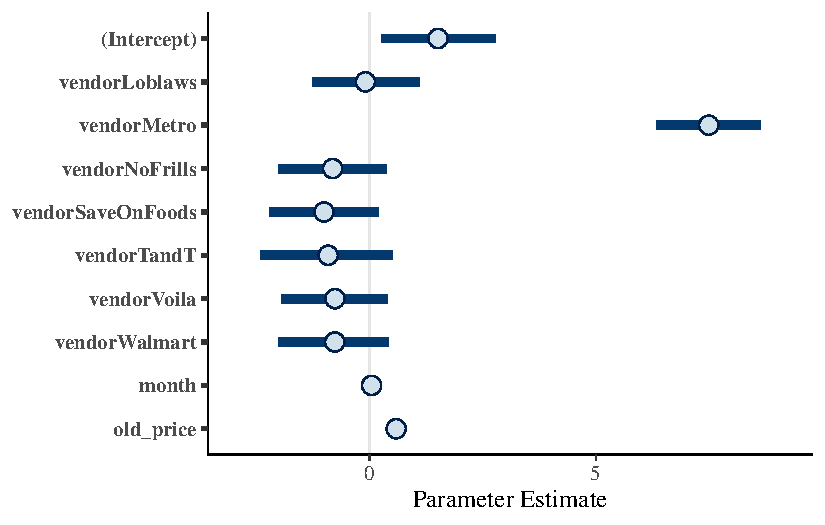
\includegraphics{paper_files/figure-pdf/fig-CI-1.pdf}

}

\caption{\label{fig-CI}Posterior Credible Intervals for Model
Parameters}

\end{figure}%

In this graph(Figure~\ref{fig-CI}), the posterior credible intervals for
the Bayesian linear regression model highlight significant differences
in strawberry pricing across vendors, seasonal trends, and the influence
of original prices. Metro stands out with a clear positive effect,
indicating its significantly higher prices compared to the reference
vendor, consistent with its premium market positioning. In contrast,
budget vendors like Save-On-Foods and No Frills exhibit negative
effects, suggesting lower pricing strategies, while other vendors show
smaller and more uncertain deviations. The positive, albeit modest,
effect of \texttt{month} suggests a slight upward trend in prices over
time, likely due to seasonal demand or inflation. The strong and precise
relationship between \texttt{old\_price} and \texttt{current\_price}
underscores the proportionality of promotional pricing strategies, where
discounts often maintain the hierarchy of original prices. Together,
these findings reveal actionable insights into vendor-specific pricing
strategies, temporal trends, and the importance of original prices in
shaping strawberry pricing dynamics.

\begin{figure}

\centering{

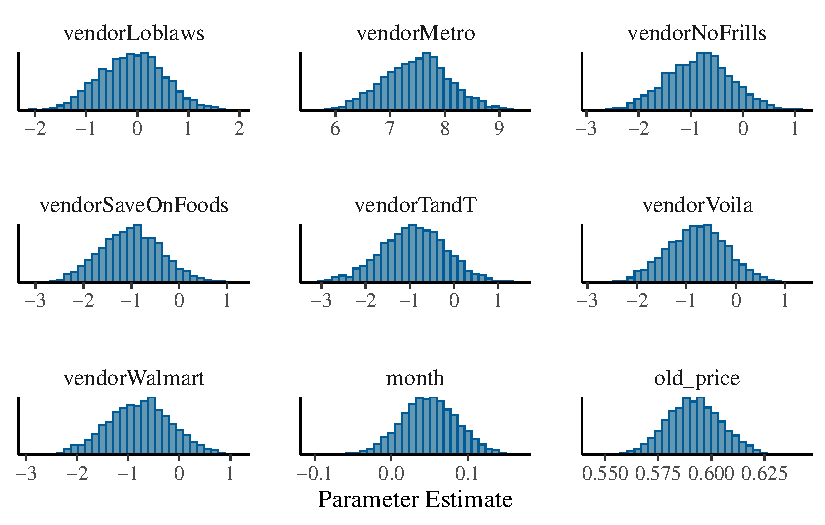
\includegraphics{paper_files/figure-pdf/fig-posterior-1.pdf}

}

\caption{\label{fig-posterior}Posterior Distribution Histograms for
Vendors and Other Parameters}

\end{figure}%

In this graph(Figure~\ref{fig-posterior}),the posterior distribution
histograms illustrate the variability in vendor pricing strategies,
temporal trends, and the influence of original prices on current
strawberry pricing. Metro's distribution is distinctly centered around a
high positive value, confirming its premium pricing strategy compared to
the reference vendor. In contrast, budget vendors like Save-On-Foods and
No Frills show distributions predominantly in the negative range,
highlighting their focus on affordability. The parameter for
\texttt{month} exhibits a narrow distribution slightly above zero,
indicating a modest upward trend in prices over time, likely driven by
seasonal fluctuations or inflation. The tightly concentrated posterior
for \texttt{old\_price} underscores its strong and consistent influence
on current prices, with higher original prices maintaining a
proportional relationship with final prices. These results emphasize the
diverse pricing strategies across vendors and the critical role of
baseline prices in shaping market dynamics.

\section{Discussion}\label{sec-discussion}

\subsection{Vendor-Specific Pricing
Strategies}\label{vendor-specific-pricing-strategies}

The analysis reveals significant differences in strawberry pricing
across vendors, highlighting how supplier identity influences retail
prices. Metro, as a premium vendor, consistently shows a positive effect
on prices compared to the reference vendor, aligning with its market
positioning that likely emphasizes quality and exclusivity. Conversely,
budget-friendly vendors such as No Frills and Save-On-Foods demonstrate
negative effects, reflecting their focus on affordability and
cost-conscious consumers. Mid-tier vendors, including Walmart and T\&T,
exhibit smaller and less consistent deviations, indicating competitive
but accessible pricing strategies. These findings suggest that
vendor-specific pricing strategies are critical in shaping market
segmentation. The implications are far-reaching: premium vendors can
continue leveraging their high-price positioning to attract niche
markets, while budget vendors might explore additional promotions to
enhance their market share. Furthermore, this variability underscores
the need for consumers to carefully consider vendor selection as a
determinant of pricing, while offering vendors opportunities to refine
strategies based on market positioning.

\subsection{Temporal Trends in
Pricing}\label{temporal-trends-in-pricing}

The study uncovers a small but positive relationship between the passage
of time (month) and strawberry prices, indicating a gradual increase in
prices over the observed period. This finding likely reflects seasonal
supply-demand dynamics, inflationary pressures, or changes in production
costs for fresh produce. While the effect is modest, it highlights the
temporal nature of pricing in retail markets and raises questions about
the drivers of these trends. Vendors may use this insight to anticipate
price increases and adjust their strategies accordingly, particularly
during periods of high demand or limited supply. For consumers, the
trend underscores the importance of seasonal awareness when planning
purchases, as prices may peak during off-seasons or holidays. The
finding also has implications for policymakers or agricultural
producers, who might explore ways to stabilize supply chains or promote
affordability during periods of high price variability. Further research
incorporating non-linear models or external factors such as weather
conditions could provide a more detailed understanding of how seasonal
patterns influence strawberry pricing.

\subsection{The Role of Original Price in Promotional
Pricing}\label{the-role-of-original-price-in-promotional-pricing}

The strong and significant relationship between old price and current
price highlights the structured nature of promotional pricing
strategies. Higher original prices are associated with proportionally
higher current prices, even after discounts or sales are applied. This
suggests that vendors maintain pricing hierarchies across their product
offerings, preserving the perceived value of premium products even
during promotional periods. For vendors, this finding underscores the
importance of setting initial prices strategically, as they serve as an
anchor for both regular and discounted pricing. For consumers, it
suggests that discounts may not always reflect deep value but instead
preserve the relative pricing order among vendors or product lines. This
structured approach to promotional pricing also indicates that vendors
likely use data-driven algorithms or market insights to optimize
discounts while maintaining brand positioning. Future research could
explore the behavioral aspects of how consumers respond to these pricing
strategies, shedding light on how perceptions of value and fairness
influence purchasing decisions during sales events.

\subsection{Weaknesses and next steps}\label{weaknesses-and-next-steps}

The Bayesian linear regression model offers a robust framework for
analyzing strawberry pricing but has notable limitations. One key
assumption is linearity, which may fail to capture non-linear or
cyclical patterns in the data, such as seasonal trends or interactions
between predictors like vendor and sale status. While interaction terms
or polynomial extensions can partially address this, more flexible
approaches like generalized additive models (GAMs) or Bayesian
hierarchical models may be better suited for complex relationships.
Additionally, the assumption of independent and identically distributed
(IID) residuals may not hold for temporal data prone to autocorrelation
or heteroscedasticity. Time-series-specific Bayesian models or robust
adjustments can help address these issues.

The reliance on priors is both a strength and a challenge. Informative
priors can stabilize estimates, especially with sparse data, but poorly
chosen priors risk biasing results. Sensitivity analysis and informed
prior selection are crucial to minimize this risk. Computational demands
are another limitation, as Bayesian methods like Markov Chain Monte
Carlo (MCMC) can be slow, especially with large datasets. Approximation
techniques like variational inference can improve speed but may
compromise precision.

Data quality is also critical. Missing, sparse, or erroneous data can
distort results, particularly for categorical variables like vendor.
Preprocessing steps such as imputation, regularization, and careful data
cleaning are essential to improve reliability. Additionally, while
posterior distributions provide nuanced probabilistic insights, they can
be challenging for non-experts to interpret. Clear communication using
visualizations and simplified summaries is necessary to make findings
actionable.

Lastly, the model struggles with scalability and extrapolation.
Predictions outside the observed data, such as for new vendors or
regions, require additional data and recalibration. The model is best
suited for interpolation within the existing dataset and should be
supplemented with external validation datasets when expanding the
analysis.

Future work can address these limitations by incorporating non-linear
models such as GAMs or Bayesian splines to better capture complex
relationships. Time-series Bayesian models can help address temporal
autocorrelation and seasonal trends. Expanding the dataset temporally
and across more vendors would enhance generalizability. Routine
sensitivity analyses and testing alternative priors can ensure robust
and unbiased results. Finally, improving stakeholder communication
through intuitive visualizations and collaboration with domain experts
will ensure that findings are both interpretable and actionable. These
steps will strengthen the Bayesian framework's ability to provide
reliable insights into strawberry pricing strategies.

\newpage

\appendix

\section*{Appendix}\label{appendix}
\addcontentsline{toc}{section}{Appendix}

\subsection{Comprehensive Data Collection Plan for Strawberry Pricing
Analysis}\label{comprehensive-data-collection-plan-for-strawberry-pricing-analysis}

\textbf{Introduction to Survey Design}

To understand strawberry pricing dynamics across Canada, a comprehensive
and robust data collection strategy is essential. This strategy combines
multiple methodologies, including web scraping, manual surveys,
partnerships with retailers, and the integration of public datasets. The
overarching aim is to ensure representativeness across geographic
regions, vendor types, and temporal variations. By collecting detailed
data, the study aims to provide actionable insights into pricing
strategies, seasonal trends, and promotional effects. Each method is
designed to address specific gaps and collectively produce a holistic
dataset that reflects the Canadian strawberry market.

\textbf{Data Collection Methods}

Web scraping will serve as the primary tool for automating data
collection from vendor websites. Websites of major grocery chains such
as Walmart, Loblaws, Metro, and Save-On-Foods will be targeted. Data
points to be extracted include product name, current price, original
price (if discounted), sale status, organic certification, and the date
of observation. Python libraries such as BeautifulSoup, Scrapy, and
Selenium will be employed to scrape structured data, which will then be
stored in a centralized database.

The scraping process will be automated to run weekly, capturing
real-time pricing updates. However, ethical and legal compliance must be
prioritized. Scraping scripts will be designed to respect the terms of
service of each website, and manual validation will be performed
periodically to ensure the accuracy of the extracted data. This method
is cost-effective, requiring a one-time investment in script development
and minimal ongoing maintenance, estimated at CAD 5,000--10,000 for
setup and CAD 1,000 per month for maintenance.

\textbf{Manual Surveys}

While web scraping provides online data, manual surveys will collect
in-store pricing information to capture physical promotions and
discrepancies between online and in-store prices. Field researchers will
visit major grocery stores, farmers' markets, and regional vendors to
record prices, sale statuses, and organic certifications. Data will be
entered into mobile-friendly platforms such as KoboToolbox or Google
Forms to minimize manual errors and enable real-time validation.

Sampling for manual surveys will focus on urban centers and suburban
areas in all Canadian provinces, with larger provinces like Ontario and
British Columbia receiving higher sampling densities. Manual surveys are
resource-intensive, with an estimated budget of CAD 20,000--30,000 to
cover wages, travel expenses, and equipment costs. Training workshops
will be conducted to ensure consistency in data collection and adherence
to protocols.

\textbf{Retailer Partnerships}

Collaborating with retailers and industry organizations will provide
access to transactional data, which includes point-of-sale (POS)
information such as pricing, sales volume, and regional variations.
Partnerships will be sought with chains like Walmart, Metro, and
Save-On-Foods, as well as the Retail Council of Canada. Data-sharing
agreements will ensure confidentiality and specify how the data will be
used.

Retailer partnerships provide high-quality, granular data but may
involve negotiation challenges and costs associated with access to
proprietary data. Agreements must outline clear data privacy policies
and address potential conflicts of interest. These partnerships can also
offer insights into customer purchasing patterns, which may supplement
the core pricing analysis.

\textbf{Public Data Repositories}

Supplementary data from public sources, such as Statistics Canada, can
contextualize the primary dataset. Variables such as regional
agricultural output, weather patterns, and population statistics will be
integrated to provide a broader understanding of pricing determinants.
Public datasets are cost-effective but may lack granularity,
necessitating careful curation and integration with primary data.

\textbf{Sampling Strategy}

To ensure the representativeness of the dataset, a stratified random
sampling approach will be used. The sampling frame will be stratified by
geography, vendor type, and time.

\textbf{Geographic Stratification}

Each province and territory will be treated as a stratum. Larger
provinces like Ontario, Quebec, and British Columbia will have higher
sample sizes due to their larger populations and market diversity. For
example: -Ontario: 300 stores (across urban and rural areas) -British
Columbia: 200 stores -Alberta: 150 stores -Smaller provinces: 50--100
stores each

\textbf{Vendor Stratification}

Vendors will be categorized into three groups: -National Chains: Large
retailers like Walmart and Loblaws. -Regional Chains: Vendors like
Save-On-Foods and Metro, which operate in specific regions. -Farmers'
Markets and Local Vendors: Smaller, independent vendors that cater to
niche markets. Sampling will ensure proportional representation from
each category, with an emphasis on national chains for broader market
insights.

\textbf{Temporal Sampling}

Data will be collected bi-weekly throughout the year to capture seasonal
trends. Special attention will be given to peak seasons (e.g., summer
harvest months) and holiday periods (e.g., Thanksgiving, Christmas) when
pricing and promotions are most dynamic.

\textbf{Data Entry and Management}

Data collected manually will be entered into Google Sheets or Excel
during the initial phase and then migrated to a centralized SQL database
or cloud storage system for processing and analysis. Web-scraped data
will directly feed into the centralized system using automated
pipelines.

Cleaning will involve:

-Removing duplicate entries. -Handling missing data through imputation
techniques (e.g., multiple imputation for continuous variables).
-Identifying outliers using statistical and visual methods (e.g.,
boxplots).

Datasets from different sources (web scraping, surveys, and
partnerships) will be merged using unique identifiers such as vendor
names and observation dates. Consistency checks will ensure uniform
formatting and variable definitions.

\textbf{Practical Considerations}

The total budget for this project is estimated at CAD 50,000--70,000.
Major cost components include personnel wages (field researchers, data
scientists), travel expenses, equipment (e.g., tablets), and data
acquisition fees from retailers.

-Web Scraping: A data scientist will develop and maintain scraping
scripts. -Manual Surveys: 10--15 field researchers will be hired and
trained. -Data Management: A project manager will oversee data
integration and quality assurance. -Collaborate with the Canadian
Ministry of Agriculture for agricultural production data. -Partner with
the Retail Council of Canada to access aggregated sales data. -Negotiate
with individual vendors for POS data access. -Ensure compliance with
data privacy laws, such as PIPEDA in Canada. -Obtain informed consent
for data sharing and usage from retailers and survey participants.

This comprehensive plan outlines a multi-method data collection strategy
that balances efficiency, cost, and representativeness. By combining web
scraping, manual surveys, retailer partnerships, and public datasets,
the project will capture the complexity of strawberry pricing dynamics
across Canada. Careful attention to sampling, legal compliance, and data
quality ensures that the collected data will support robust analysis and
actionable insights. This integrated approach provides a solid
foundation for understanding market trends and guiding vendor and
consumer decisions.

\subsection{Comprehensive Data Analysis Plan for Strawberry Pricing
Dynamics}\label{comprehensive-data-analysis-plan-for-strawberry-pricing-dynamics}

\textbf{Overview of Analysis Plan} After collecting the strawberry
pricing data, the next step involves applying specific analysis methods
to uncover key insights into vendor pricing strategies, seasonal trends,
and the impact of promotions. The primary analysis will use a Bayesian
linear regression model, supplemented by exploratory data analysis
(EDA), diagnostic checks, and predictive performance evaluations. Each
method and its implementation is described in detail below, along with a
discussion of its strengths, limitations, and areas for improvement.

\textbf{Exploratory Data Analysis (EDA)}

Exploratory Data Analysis (EDA) serves as the foundation for
understanding the dataset, identifying patterns, and detecting potential
issues before applying advanced models. Visualization techniques such as
boxplots, histograms, and line plots will reveal distributions and
trends in key variables like \texttt{current\_price},
\texttt{old\_price}, and \texttt{month}. For example, boxplots comparing
prices across vendors will highlight vendor-specific pricing strategies,
while line plots will uncover temporal trends, including seasonal
variations in strawberry prices. Summary statistics, such as the mean
and median of prices per vendor or region, will provide an overview of
central tendencies and variability. Correlation matrices will also help
identify relationships between variables, such as the association
between original and discounted prices.

While EDA provides critical insights, its reliance on visual and
descriptive methods limits its ability to quantify relationships or
infer causality. Nevertheless, it is an essential first step that
ensures data quality and informs subsequent modeling decisions.
Potential issues, such as missing values or outliers, identified during
EDA, will be addressed through imputation techniques and robust
statistical methods.

\textbf{Bayesian Linear Regression Model}

The primary analysis method is a Bayesian linear regression model,
chosen for its flexibility and ability to incorporate prior knowledge
while providing robust parameter estimates. The model will quantify the
effects of predictors such as vendor (\texttt{vendor}), sale status
(\texttt{sale\_status}), temporal trends (\texttt{month}), and original
price (\texttt{old\_price}) on the current price of strawberries
(\texttt{current\_price}). The model will include the following
structure:

{[} y\_i = \beta\emph{0 + \beta}\{\text{vendor}{[}i{]}\} +
\beta\emph{\{\text{organic}\} \cdot x}\{\text{organic}{[}i{]}\} +
\beta\emph{\{\text{sale}\} \cdot x}\{\text{sale}{[}i{]}\} +
\beta\emph{\{\text{month}\} \cdot x}\{\text{month}{[}i{]}\} +
\beta\emph{\{\text{old\_price}\} \cdot x}\{\text{old\_price}{[}i{]}\} +
\epsilon\_i {]}

Each coefficient (\(\beta\)) will have a prior distribution, such as a
normal prior centered at zero, reflecting initial uncertainty about its
effect. For instance, the prior for \(\beta_{\text{vendor}}\) assumes no
significant differences between vendors initially, allowing the data to
dominate posterior estimates. The Bayesian framework also provides
posterior distributions for each parameter, which capture uncertainty
and enable credible intervals for inference. For example, a 95\%
credible interval for \(\beta_{\text{old\_price}}\) indicates the range
of plausible values for the effect of original prices on current prices,
accounting for uncertainty.

The Bayesian approach offers significant advantages, including the
ability to stabilize estimates for predictors with limited observations
and provide probabilistic interpretations of results. However, it
requires careful selection of priors, as overly informative priors may
bias the results, while uninformative priors may weaken the model's
ability to draw meaningful conclusions. The computational demands of
Bayesian modeling are another limitation, particularly for large
datasets, but this can be addressed through parallel processing or
variational inference methods.

\textbf{Diagnostic Checks and Model Validation}

Model diagnostics are critical to ensuring that the Bayesian regression
model fits the data well and produces reliable estimates. Posterior
predictive checks (pp\_checks) will compare observed data with simulated
data from the model to evaluate its ability to replicate the observed
distribution of prices. For instance, discrepancies between the
predicted and observed distributions may indicate model
misspecifications or missing predictors.

Trace plots will be used to examine the convergence of Markov Chain
Monte Carlo (MCMC) sampling for each parameter, ensuring that the chains
are stationary and mixing well. Rhat values, which assess convergence
across chains, must be close to 1.0 for all parameters. Residual
analysis will identify potential violations of assumptions, such as
heteroscedasticity or autocorrelation, which may require model
adjustments.

Model validation will include leave-one-out cross-validation (LOO-CV) to
evaluate predictive performance and compare alternative models. For
example, LOO-CV can confirm whether including interaction terms (e.g.,
vendor and sale status) improves the model's ability to predict prices.
Metrics like root mean square error (RMSE) will quantify the average
deviation between observed and predicted prices, providing a measure of
overall model fit.

While these diagnostics enhance the robustness of the analysis, they
require significant computational resources and expertise to interpret.
Incorporating automated diagnostic tools, such as those provided by the
\textbf{bayesplot} package, can streamline this process and improve
efficiency.

\textbf{Predictive Analysis and Simulations}

Beyond inference, the Bayesian regression model will be used for
predictive analysis to assess the model's real-world applicability.
Simulations will explore hypothetical scenarios, such as the effect of a
uniform 10\% discount across all vendors, to predict how pricing
strategies might shift and impact consumer behavior. Temporal trends can
also be analyzed by simulating seasonal effects, such as price
fluctuations during peak harvest months or holiday periods.

Predictive accuracy will be evaluated using observed holdout data to
ensure the model generalizes well to unseen scenarios. Comparisons with
alternative methods, such as generalized additive models (GAMs) or
random forests, will provide additional validation. Simulations offer
valuable insights for stakeholders, such as how adjusting promotional
strategies might influence market share, but they depend heavily on the
quality of input data and assumptions about unobserved factors.

\textbf{Limitations and Areas for Improvement}

The analysis methods have inherent limitations. Bayesian regression
assumes linear relationships between predictors and outcomes, which may
not capture non-linear trends or complex interactions. Extending the
model to include interaction terms or adopting more flexible approaches,
such as GAMs, can address this limitation. The reliance on priors, while
a strength in stabilizing estimates, introduces the risk of bias if
priors are not chosen carefully. Sensitivity analysis is crucial to
ensure that results are robust to changes in prior specifications.

Another limitation is the potential for unobserved confounders, such as
geographic factors or consumer preferences, which may bias estimates.
Collecting additional variables, such as store location or customer
demographics, could improve the model's explanatory power. Computational
demands are also a challenge, particularly for large datasets or complex
models. Using high-performance computing resources or approximate
inference methods can mitigate these issues.

The data analysis plan integrates EDA, Bayesian linear regression,
diagnostic checks, and predictive analysis to provide a comprehensive
understanding of strawberry pricing dynamics. While the Bayesian
approach offers robust and probabilistic insights, it requires careful
attention to prior selection, diagnostics, and computational efficiency.
The combination of rigorous modeling and scenario-based simulations
ensures actionable insights for stakeholders, including vendors and
consumers. Future improvements, such as incorporating additional
predictors or testing non-linear models, can further enhance the
analysis and its applicability to real-world pricing strategies.

\subsection{Additional data details}\label{additional-data-details}

Table~\ref{tbl-skim} shows a summary of the analysis dataset.

\begin{table}

\caption{\label{tbl-skim}Summary Statistics and Distribution Overview of
the Analysis Dataset}

\centering{

\centering
\begin{tblr}[         %% tabularray outer open
]                     %% tabularray outer close
{                     %% tabularray inner open
colspec={Q[]Q[]Q[]Q[]Q[]Q[]Q[]Q[]Q[]},
hline{5}={1,2,3,4,5,6,7,8,9}{solid, 0.1em, black},
}                     %% tabularray inner close
\toprule
& Unique & Missing Pct. & Mean & SD & Min & Median & Max & Histogram \\ \midrule %% TinyTableHeader
current\_price & 238 & 0 & 7.8 & 12.7 & 0.0 & 5.0 & 290.0 & 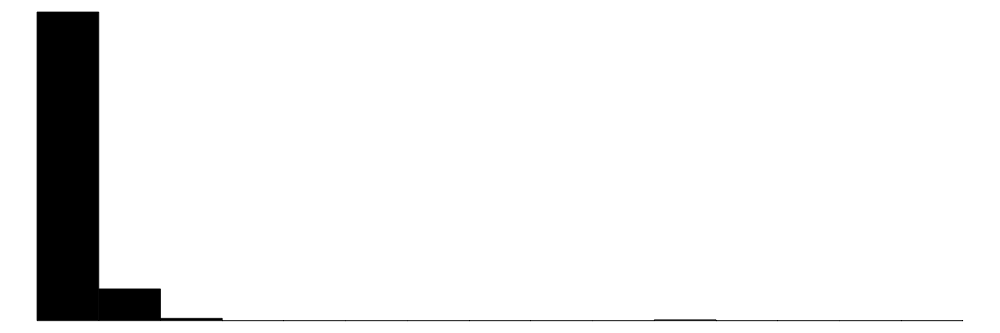
\includegraphics[height=1em]{tinytable_assets/idipy3vtsc1mlpgxt8o3o7.png} \\
old\_price & 200 & 0 & 6.1 & 4.3 & 0.4 & 5.4 & 348.0 & 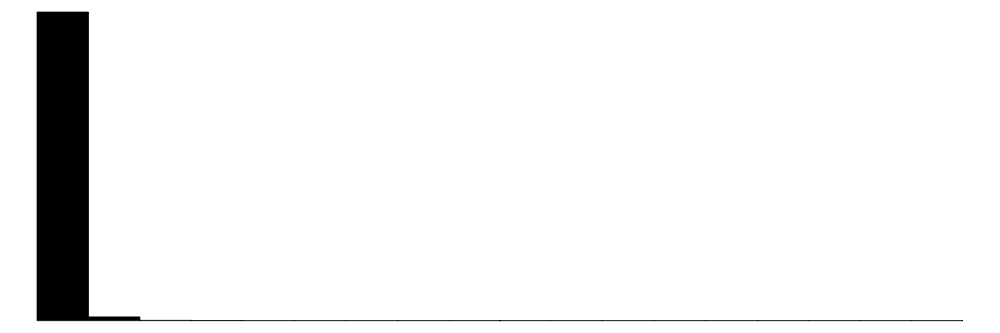
\includegraphics[height=1em]{tinytable_assets/idp1xv0vuvfk5ug1wh0mm9.png} \\
month & 8 & 0 & 8.9 & 1.6 & 4.0 & 9.0 & 11.0 & 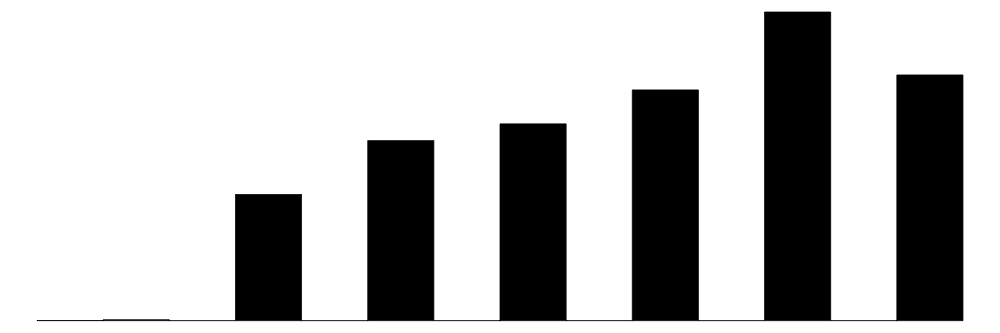
\includegraphics[height=1em]{tinytable_assets/idoylf132wx8wev5gteo4b.png} \\
vendor & N & \% &  &  &  &  &  &  \\
Galleria & 400 & 0.9 &  &  &  &  &  &  \\
Loblaws & 4595 & 10.2 &  &  &  &  &  &  \\
Metro & 15819 & 35.3 &  &  &  &  &  &  \\
NoFrills & 4203 & 9.4 &  &  &  &  &  &  \\
SaveOnFoods & 4531 & 10.1 &  &  &  &  &  &  \\
TandT & 627 & 1.4 &  &  &  &  &  &  \\
Voila & 10549 & 23.5 &  &  &  &  &  &  \\
Walmart & 4130 & 9.2 &  &  &  &  &  &  \\
\bottomrule
\end{tblr}

}

\end{table}%

\textbf{Data Source and Cleaning Process}

The data for this study comes from the Project Hammer website, an open
data platform centered on grocery prices from multiple suppliers in
Canada. The platform captures multidimensional data including product
prices, supplier information, promotional discounts, etc. through web
scraping technology, and combines manual verification to ensure its
reliability. These data provide price dynamics in different regions and
suppliers in Canada, laying the foundation for studying the fluctuations
and market strategies of strawberry prices.

In order to meet the analysis needs, the data was cleaned in multiple
steps. First, the rows with missing values in the current price and old
price variables were deleted because these prices are the core of the
study. If the price records are incomplete, the analysis results will be
distorted. In addition, for the vendor and month variables, it was
confirmed that there were no missing values to ensure the integrity of
the supplier and time information.

Secondly, the interquartile range (IQR) method was used to detect and
process outliers. The focus of the cleaning was on identifying and
eliminating possible entry errors (such as extremely low or high
prices). However, legitimate outliers (such as high prices for high-end
strawberries) were retained to ensure the authenticity of the data. At
the same time, all price fields were standardized and prices were
recorded uniformly as the price per pound of strawberries to facilitate
horizontal comparison between suppliers.

\textbf{The strengths and limitations of data}

On the plus side, the data is diverse, covering both national and
regional suppliers, including Voila, Metro, and Walmart, among others.
This provides a unique perspective on the differences between different
market positioning and pricing strategies. In addition, the data cover
observations across multiple months, providing a solid basis for
exploring seasonal fluctuations in strawberry prices. Simultaneous
recording of the price variables current price and old price allows
studying the impact of discount and promotion strategies on the final
price.

Although the data has significant advantages, there are also some
limitations. First, the data focuses primarily on urban and suburban
providers, and pricing trends in rural areas may be understated. Second,
web scraping technology captures static snapshots and is difficult to
record real-time price fluctuations, such as flash sales or limited-time
discounts. In addition, some records lack explicit promotion status
markers (such as whether the product is discounted), which limits
detailed analysis of discount strategies. Finally, the density of
records across months may be uneven across different providers, which
may introduce bias in the temporal analysis.

\textbf{Data Analysis Outlook}

Based on the cleaned data, the analysis can focus on several key
directions. First, by combining the current price and old price
variables, we can delve into the impact of promotions on pricing
strategies. For example, we can quantify the magnitude of price
fluctuations during promotions for different suppliers and their
potential impact on consumer behavior. Second, through the month
variable, we can capture the seasonal fluctuations in strawberry prices.
This will help us understand how supply and demand adjust with seasonal
changes and provide an important basis for predicting future price
trends.

In addition, using the vendor variable, we can compare the pricing
strategies of different suppliers. The study may reveal whether high-end
suppliers (such as Metro) are positioned in the high-end market through
higher prices, while low-price suppliers (such as Walmart and
Save-On-Foods) attract more price-sensitive consumers through discounts.
These findings will provide in-depth insights into understanding the
dynamics of the Canadian strawberry market, while providing data support
for policymakers and retailers to optimize market strategies.

Overall, the cleaned dataset provides a valuable resource for in-depth
study of strawberry price fluctuations and supplier strategies. Despite
limitations such as geographic coverage bias and insufficient capture of
dynamic prices, the diversity and time span of the data ensure the wide
applicability of the analysis. By combining the analysis of promotions,
seasonal fluctuations, and supplier differences, the study reveals
complex pricing patterns and competitive strategies in the Canadian
market.

\subsection{Further Background Details and Diagnostics of the
Model}\label{sec-model-details}

\textbf{Model Background and Justification}

The Bayesian linear regression model provides a probabilistic framework
to understand the determinants of strawberry pricing across Canadian
vendors. This model was chosen for its ability to incorporate prior
knowledge, handle parameter uncertainty, and deliver intuitive,
probabilistic interpretations of results. Unlike traditional frequentist
regression, Bayesian regression generates posterior distributions for
all parameters, offering insights into the uncertainty and variability
of each predictor's effect.

The primary dependent variable in the model is \texttt{current\_price},
representing the observed price per pound of strawberries. Key
predictors include vendor identity (\(\text{vendor}\)), original price
(\(\text{old\_price}\)), sale status (\(\text{sale\_status}\)), and
temporal trends (\(\text{month}\)). These variables capture the diverse
factors influencing pricing, such as competitive strategies among
vendors, promotional effects, and seasonal supply-demand dynamics.

The model specification includes normal priors for regression
coefficients (\(\beta\)) and an exponential prior for the residual
standard deviation (\(\sigma\)). This setup reflects reasonable
assumptions about the effects of predictors, such as small, centered
effects with moderate variability. For instance, the prior for
\(\beta_{\text{vendor}}\) assumes no extreme pricing differences between
vendors, while allowing the data to dominate posterior updates.

\textbf{Model Diagnostics and Validation}

Posterior predictive checks compare the observed distribution of
\texttt{current\_price} with simulated data generated from the model.
The goal is to assess whether the model adequately captures the
variability and central tendencies of the observed data. For this
analysis, posterior predictive plots revealed close alignment between
observed and predicted prices, indicating a good fit. Minor
discrepancies at the tails suggest that the model may not fully capture
extreme price outliers, which could be addressed by adding robust
regression components or alternative distributions.

In Figure~\ref{fig-ppcheckandposteriorvsprior-1} we implement a
posterior predictive check. The posterior predictive check (pp\_check)
graph compares the observed strawberry prices (\texttt{y}) with the
predicted prices (\texttt{y\_rep}) generated by the Bayesian linear
regression model, revealing both strengths and limitations of the
model's fit. The model captures the overall trend of lower prices
reasonably well, as indicated by the alignment of the observed and
predicted densities in the left portion of the graph. However,
discrepancies arise at higher price points, where the predicted density
smooths over the sharp peaks and variability present in the observed
data. This suggests that while the model performs adequately for most
data points, it struggles to represent the complexity of premium
pricing, possibly due to missing predictors or oversimplified
assumptions about linearity. These findings highlight the need for
further refinement, such as incorporating additional factors or
exploring non-linear relationships, to improve the model's ability to
account for variability in higher-priced strawberries.

In Figure~\ref{fig-ppcheckandposteriorvsprior-2} we compare the
posterior with the prior. The posterior vs.~prior graph illustrates how
the Bayesian model updates parameter estimates by integrating observed
data with prior assumptions. For key predictors such as
\texttt{vendorMetro} and \texttt{old\_price}, the posterior
distributions show significant shifts away from the priors, indicating
strong evidence from the data and high confidence in these parameters'
effects. In contrast, parameters like \texttt{vendorWalmart} and
\texttt{vendorTandT} have posterior distributions that remain closer to
the priors, reflecting weaker or less conclusive effects. The priors,
which were set to be uninformative and centered around zero, allowed the
data to dominate the posterior estimates where evidence was strong,
while providing a baseline for parameters with less evidence. This
balance highlights the Bayesian framework's ability to refine parameter
estimates, narrow uncertainty for influential predictors, and maintain
flexibility where the data provides limited information. Overall, the
graph emphasizes the robustness and nuance of Bayesian inference in
capturing vendor-specific pricing strategies and other predictors.

\begin{figure}

\begin{minipage}{0.50\linewidth}

\centering{

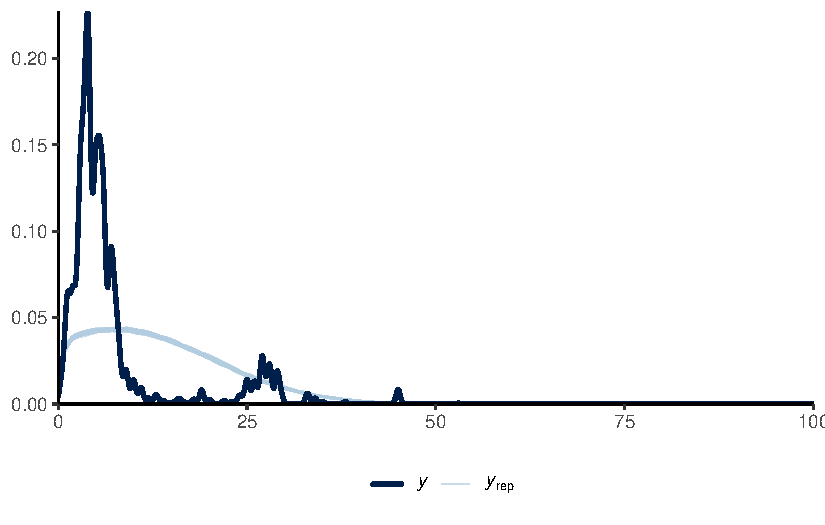
\includegraphics{paper_files/figure-pdf/fig-ppcheckandposteriorvsprior-1.pdf}

}

\subcaption{\label{fig-ppcheckandposteriorvsprior-1}Posterior prediction
check}

\end{minipage}%
%
\begin{minipage}{0.50\linewidth}

\centering{

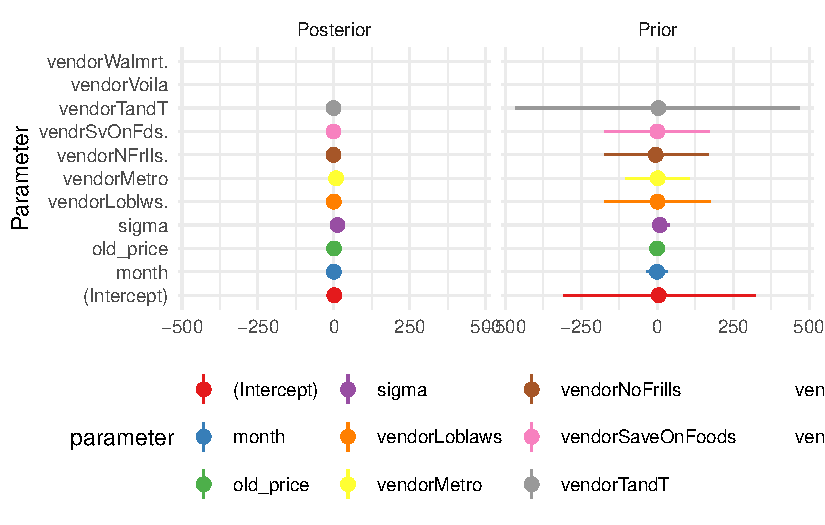
\includegraphics{paper_files/figure-pdf/fig-ppcheckandposteriorvsprior-2.pdf}

}

\subcaption{\label{fig-ppcheckandposteriorvsprior-2}Comparing the
posterior with the prior}

\end{minipage}%

\caption{\label{fig-ppcheckandposteriorvsprior}Examining how the model
fits, and is affected by, the data}

\end{figure}%

Trace plots visualize the behavior of the Markov Chain Monte Carlo
(MCMC) sampling process for each parameter. Convergence is achieved when
chains are stationary and overlap across iterations. For this model,
trace plots showed consistent mixing and no evidence of divergence,
confirming that the chains have converged and are exploring the
posterior distributions effectively. The Rhat statistic evaluates chain
convergence across parallel MCMC simulations. All Rhat values for the
parameters in this model were close to 1.0, indicating excellent
convergence. This result provides confidence that the posterior
distributions are reliable and free from sampling biases.

Figure~\ref{fig-stanareyouokay-1} is a trace plot. The trace plot
illustrates the behavior of the MCMC sampling process for each parameter
in the Bayesian linear regression model, confirming convergence and
proper mixing across four chains. The overlapping and stationary
patterns of the chains indicate that the sampler has stabilized and is
efficiently exploring the posterior distributions. Parameters like
\texttt{vendorMetro} and \texttt{old\_price} show tightly grouped
traces, reflecting high confidence in their estimates, while greater
variability in parameters such as \texttt{vendorLoblaws} suggests less
certainty, possibly due to weaker relationships or data limitations. The
absence of trends or gaps in the traces supports the reliability of the
sampling process, ensuring that the posterior estimates are robust and
representative of the underlying data. This provides confidence in the
model's results and its ability to capture the factors influencing
strawberry pricing effectively.

Figure~\ref{fig-stanareyouokay-2} is a Rhat plot. The Rhat plot
demonstrates excellent convergence for all parameters in the Bayesian
linear regression model, with Rhat values close to 1 across the board.
This indicates that the MCMC chains have mixed well and are sampling
from the same posterior distribution, ensuring reliable and unbiased
parameter estimates. The absence of any parameters with Rhat values
exceeding critical thresholds (e.g., 1.05 or 1.1) confirms that the
sampling process was efficient and sufficient, requiring no additional
iterations or model adjustments. This strong convergence provides
confidence in the robustness and reproducibility of the posterior
estimates, supporting the validity of the model's findings in analyzing
strawberry pricing dynamics.

\begin{figure}

\begin{minipage}{0.50\linewidth}

\centering{

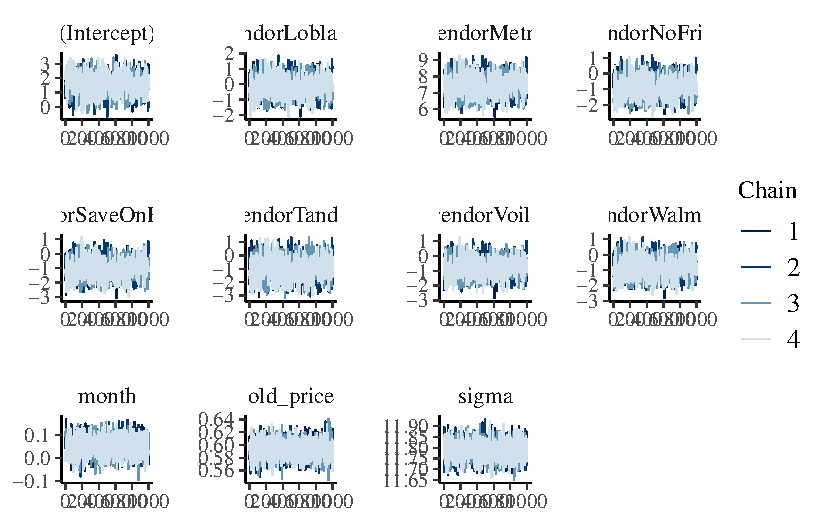
\includegraphics{paper_files/figure-pdf/fig-stanareyouokay-1.pdf}

}

\subcaption{\label{fig-stanareyouokay-1}Trace plot}

\end{minipage}%
%
\begin{minipage}{0.50\linewidth}

\centering{

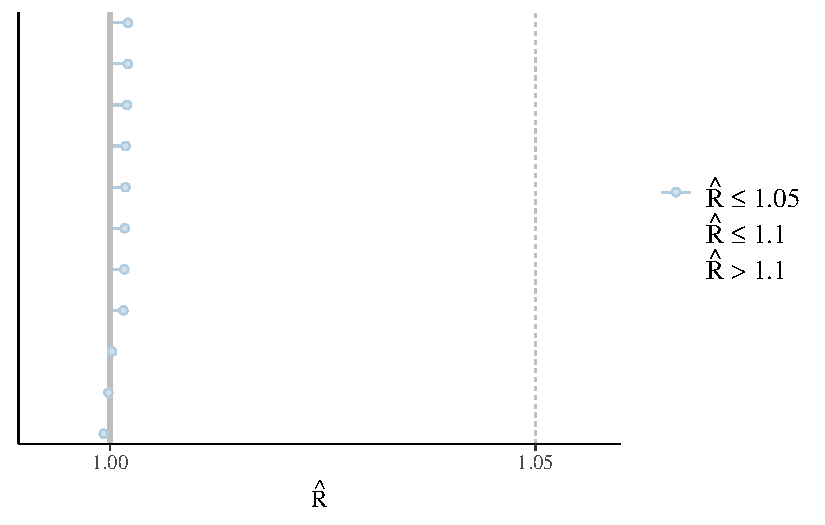
\includegraphics{paper_files/figure-pdf/fig-stanareyouokay-2.pdf}

}

\subcaption{\label{fig-stanareyouokay-2}Rhat plot}

\end{minipage}%

\caption{\label{fig-stanareyouokay}Checking the convergence of the MCMC
algorithm}

\end{figure}%

\textbf{Model Fit Metrics}

\begin{itemize}
\item
  \textbf{( R\^{}2 )} and \textbf{Adjusted ( R\^{}2 )}: The model
  explained approximately 13.9\% of the variance in strawberry prices,
  reflecting the complexity of pricing dynamics influenced by unobserved
  factors like geographic location and consumer preferences.
\item
  \textbf{Root Mean Square Error (RMSE)}: An RMSE of 11.79 indicates
  moderate predictive accuracy, which aligns with expectations given the
  variability in pricing strategies across vendors.
\item
  \textbf{Leave-One-Out Cross-Validation (LOO-CV)}: The LOO-CV score
  confirmed the model's predictive consistency and supported its
  suitability for analyzing strawberry pricing.
\end{itemize}

\newpage

\section*{References}\label{references}
\addcontentsline{toc}{section}{References}

\phantomsection\label{refs}
\begin{CSLReferences}{1}{0}
\bibitem[\citeproctext]{ref-arrow}
Apache Arrow. 2021. \emph{{arrow: Integration to 'Apache' 'Arrow'}}.
\url{https://CRAN.R-project.org/package=arrow}.

\bibitem[\citeproctext]{ref-modelsummary}
Arel-Bundock, Vincent. 2022. {``{modelsummary}: Data and Model Summaries
in {R}.''} \emph{Journal of Statistical Software} 103 (1): 1--23.
\url{https://doi.org/10.18637/jss.v103.i01}.

\bibitem[\citeproctext]{ref-filipp2024hammer}
Filipp, Jacob. 2024. {``Hammer - a Modern Statistical Computing Tool.''}
\url{https://jacobfilipp.com/hammer/}.

\bibitem[\citeproctext]{ref-bayesplot}
Gelman, Gabriel, Jonah Gabry, et al. 2021. \emph{{bayesplot: Plotting
for Bayesian Models}}. \url{https://mc-stan.org/bayesplot}.

\bibitem[\citeproctext]{ref-rstanarm}
Goodrich, Ben, Jonah Gabry, Imad Ali, and Sam Brilleman. 2022.
{``{rstanarm: {Bayesian} applied regression modeling via {Stan}}.''}
\url{https://mc-stan.org/rstanarm/}.

\bibitem[\citeproctext]{ref-hodgdon2024current}
Hodgdon, Elisabeth A, David S Conner, Laura G McDermott, Marvin P
Pritts, David T Handley, Kaitlyn M Orde, and Rebecca Grube Sideman.
2024. {``A Current View on Strawberry Production Practices and Trends in
the Northeastern United States and Canada.''} \emph{HortTechnology} 34
(5): 574--84.

\bibitem[\citeproctext]{ref-macoun1919strawberry}
Macoun, William Tyrrell, and WA McCubbin. 1919. \emph{The Strawberry and
Its Cultivation in Canada}. Department of Agriculture.

\bibitem[\citeproctext]{ref-here}
Müller, Kirill. 2020. \emph{Here: A Simpler Way to Find Your Files}.
\url{https://CRAN.R-project.org/package=here}.

\bibitem[\citeproctext]{ref-citeR}
R Core Team. 2023. \emph{{R: A Language and Environment for Statistical
Computing}}. Vienna, Austria: R Foundation for Statistical Computing.
\url{https://www.R-project.org/}.

\bibitem[\citeproctext]{ref-testthat}
Wickham, Hadley. 2011. {``Testthat: Get Started with Testing.''}
\emph{The R Journal} 3: 5--10.
\url{https://journal.r-project.org/archive/2011-1/RJournal_2011-1_Wickham.pdf}.

\bibitem[\citeproctext]{ref-tidyverse}
Wickham, Hadley, Mara Averick, Jennifer Bryan, Winston Chang, Lucy
D'Agostino McGowan, Romain François, Garrett Grolemund, et al. 2019.
{``Welcome to the {tidyverse}.''} \emph{Journal of Open Source Software}
4 (43): 1686. \url{https://doi.org/10.21105/joss.01686}.

\bibitem[\citeproctext]{ref-knitr}
Xie, Yihui. 2021. \emph{{knitr: A General-Purpose Package for Dynamic
Report Generation in R}}. \url{https://yihui.org/knitr/}.

\end{CSLReferences}




\end{document}
